
%% bare_conf.tex
%% V1.4
%% 2012/12/27
%% by Michael Shell
%% See:
%% http://www.michaelshell.org/
%% for current contact information.
%%
%% This is a skeleton file demonstrating the use of IEEEtran.cls
%% (requires IEEEtran.cls version 1.8 or later) with an IEEE conference paper.
%%
%% Support sites:
%% http://www.michaelshell.org/tex/ieeetran/
%% http://www.ctan.org/tex-archive/macros/latex/contrib/IEEEtran/
%% and
%% http://www.ieee.org/

%%*************************************************************************
%% Legal Notice:
%% This code is offered as-is without any warranty either expressed or
%% implied; without even the implied warranty of MERCHANTABILITY or
%% FITNESS FOR A PARTICULAR PURPOSE! 
%% User assumes all risk.
%% In no event shall IEEE or any contributor to this code be liable for
%% any damages or losses, including, but not limited to, incidental,
%% consequential, or any other damages, resulting from the use or misuse
%% of any information contained here.
%%
%% All comments are the opinions of their respective authors and are not
%% necessarily endorsed by the IEEE.
%%
%% This work is distributed under the LaTeX Project Public License (LPPL)
%% ( http://www.latex-project.org/ ) version 1.3, and may be freely used,
%% distributed and modified. A copy of the LPPL, version 1.3, is included
%% in the base LaTeX documentation of all distributions of LaTeX released
%% 2003/12/01 or later.
%% Retain all contribution notices and credits.
%% ** Modified files should be clearly indicated as such, including  **
%% ** renaming them and changing author support contact information. **
%%
%% File list of work: IEEEtran.cls, IEEEtran_HOWTO.pdf, bare_adv.tex,
%%                    bare_conf.tex, bare_jrnl.tex, bare_jrnl_compsoc.tex,
%%                    bare_jrnl_transmag.tex
%%*************************************************************************

% *** Authors should verify (and, if needed, correct) their LaTeX system  ***
% *** with the testflow diagnostic prior to trusting their LaTeX platform ***
% *** with production work. IEEE's font choices can trigger bugs that do  ***
% *** not appear when using other class files.                            ***
% The testflow support page is at:
% http://www.michaelshell.org/tex/testflow/



% Note that the a4paper option is mainly intended so that authors in
% countries using A4 can easily print to A4 and see how their papers will
% look in print - the typesetting of the document will not typically be
% affected with changes in paper size (but the bottom and side margins will).
% Use the testflow package mentioned above to verify correct handling of
% both paper sizes by the user's LaTeX system.
%
% Also note that the "draftcls" or "draftclsnofoot", not "draft", option
% should be used if it is desired that the figures are to be displayed in
% draft mode.
%
\documentclass[12pt,a4paper,final]{article}
% Add the compsoc option for Computer Society conferences.
%
% If IEEEtran.cls has not been installed into the LaTeX system files,
% manually specify the path to it like:
\usepackage[latin1]{inputenc}
\usepackage{amsfonts}
\usepackage{amssymb}
\usepackage{amsthm}
\usepackage{fullpage}
\usepackage{setspace}
\usepackage{graphicx}
%\usepackage[pdftex]{graphicx}
\usepackage{psfrag}
\usepackage{color}
\usepackage{epsfig}
\usepackage{appendix}
\usepackage{caption}
\usepackage{cite}
\usepackage{ifpdf}
\usepackage[cmex10]{amsmath}
\usepackage{algorithmic}
\usepackage{array}
\usepackage{stfloats}
\usepackage{url}
\usepackage{fixltx2e}
\usepackage{setspace} 
\usepackage{diagbox}





% Some very useful LaTeX packages include:
% (uncomment the ones you want to load)


% *** MISC UTILITY PACKAGES ***
%
%\usepackage{ifpdf}
% Heiko Oberdiek's ifpdf.sty is very useful if you need conditional
% compilation based on whether the output is pdf or dvi.
% usage:
% \ifpdf
%   % pdf code
% \else
%   % dvi code
% \fi
% The latest version of ifpdf.sty can be obtained from:
% http://www.ctan.org/tex-archive/macros/latex/contrib/oberdiek/
% Also, note that IEEEtran.cls V1.7 and later provides a builtin
% \ifCLASSINFOpdf conditional that works the same way.
% When switching from latex to pdflatex and vice-versa, the compiler may
% have to be run twice to clear warning/error messages.






% *** CITATION PACKAGES ***
%
%\usepackage{cite}
% cite.sty was written by Donald Arseneau
% V1.6 and later of IEEEtran pre-defines the format of the cite.sty package
% \cite{} output to follow that of IEEE. Loading the cite package will
% result in citation numbers being automatically sorted and properly
% "compressed/ranged". e.g., [1], [9], [2], [7], [5], [6] without using
% cite.sty will become [1], [2], [5]--[7], [9] using cite.sty. cite.sty's
% \cite will automatically add leading space, if needed. Use cite.sty's
% noadjust option (cite.sty V3.8 and later) if you want to turn this off
% such as if a citation ever needs to be enclosed in parenthesis.
% cite.sty is already installed on most LaTeX systems. Be sure and use
% version 4.0 (2003-05-27) and later if using hyperref.sty. cite.sty does
% not currently provide for hyperlinked citations.
% The latest version can be obtained at:
% http://www.ctan.org/tex-archive/macros/latex/contrib/cite/
% The documentation is contained in the cite.sty file itself.






% *** GRAPHICS RELATED PACKAGES ***
%
%\ifCLASSINFOpdf
  % \usepackage[pdftex]{graphicx}
  % declare the path(s) where your graphic files are
  % \graphicspath{{../pdf/}{../jpeg/}}
  % and their extensions so you won't have to specify these with
  % every instance of \includegraphics
  % \DeclareGraphicsExtensions{.pdf,.jpeg,.png}
%\else
  % or other class option (dvipsone, dvipdf, if not using dvips). graphicx
  % will default to the driver specified in the system graphics.cfg if no
  % driver is specified.
  % \usepackage[dvips]{graphicx}
  % declare the path(s) where your graphic files are
  % \graphicspath{{../eps/}}
  % and their extensions so you won't have to specify these with
  % every instance of \includegraphics
  % \DeclareGraphicsExtensions{.eps}
%\fi
% graphicx was written by David Carlisle and Sebastian Rahtz. It is
% required if you want graphics, photos, etc. graphicx.sty is already
% installed on most LaTeX systems. The latest version and documentation
% can be obtained at: 
% http://www.ctan.org/tex-archive/macros/latex/required/graphics/
% Another good source of documentation is "Using Imported Graphics in
% LaTeX2e" by Keith Reckdahl which can be found at:
% http://www.ctan.org/tex-archive/info/epslatex/
%
% latex, and pdflatex in dvi mode, support graphics in encapsulated
% postscript (.eps) format. pdflatex in pdf mode supports graphics
% in .pdf, .jpeg, .png and .mps (metapost) formats. Users should ensure
% that all non-photo figures use a vector format (.eps, .pdf, .mps) and
% not a bitmapped formats (.jpeg, .png). IEEE frowns on bitmapped formats
% which can result in "jaggedy"/blurry rendering of lines and letters as
% well as large increases in file sizes.
%
% You can find documentation about the pdfTeX application at:
% http://www.tug.org/applications/pdftex





% *** MATH PACKAGES ***
%
%\usepackage[cmex10]{amsmath}
% A popular package from the American Mathematical Society that provides
% many useful and powerful commands for dealing with mathematics. If using
% it, be sure to load this package with the cmex10 option to ensure that
% only type 1 fonts will utilized at all point sizes. Without this option,
% it is possible that some math symbols, particularly those within
% footnotes, will be rendered in bitmap form which will result in a
% document that can not be IEEE Xplore compliant!
%
% Also, note that the amsmath package sets \interdisplaylinepenalty to 10000
% thus preventing page breaks from occurring within multiline equations. Use:
%\interdisplaylinepenalty=2500
% after loading amsmath to restore such page breaks as IEEEtran.cls normally
% does. amsmath.sty is already installed on most LaTeX systems. The latest
% version and documentation can be obtained at:
% http://www.ctan.org/tex-archive/macros/latex/required/amslatex/math/





% *** SPECIALIZED LIST PACKAGES ***
%
%\usepackage{algorithmic}
% algorithmic.sty was written by Peter Williams and Rogerio Brito.
% This package provides an algorithmic environment fo describing algorithms.
% You can use the algorithmic environment in-text or within a figure
% environment to provide for a floating algorithm. Do NOT use the algorithm
% floating environment provided by algorithm.sty (by the same authors) or
% algorithm2e.sty (by Christophe Fiorio) as IEEE does not use dedicated
% algorithm float types and packages that provide these will not provide
% correct IEEE style captions. The latest version and documentation of
% algorithmic.sty can be obtained at:
% http://www.ctan.org/tex-archive/macros/latex/contrib/algorithms/
% There is also a support site at:
% http://algorithms.berlios.de/index.html
% Also of interest may be the (relatively newer and more customizable)
% algorithmicx.sty package by Szasz Janos:
% http://www.ctan.org/tex-archive/macros/latex/contrib/algorithmicx/




% *** ALIGNMENT PACKAGES ***
%
%\usepackage{array}
% Frank Mittelbach's and David Carlisle's array.sty patches and improves
% the standard LaTeX2e array and tabular environments to provide better
% appearance and additional user controls. As the default LaTeX2e table
% generation code is lacking to the point of almost being broken with
% respect to the quality of the end results, all users are strongly
% advised to use an enhanced (at the very least that provided by array.sty)
% set of table tools. array.sty is already installed on most systems. The
% latest version and documentation can be obtained at:
% http://www.ctan.org/tex-archive/macros/latex/required/tools/


% IEEEtran contains the IEEEeqnarray family of commands that can be used to
% generate multiline equations as well as matrices, tables, etc., of high
% quality.




% *** SUBFIGURE PACKAGES ***
%\ifCLASSOPTIONcompsoc
%  \usepackage[caption=false,font=normalsize,labelfont=sf,textfont=sf]{subfig}
%\else
%  \usepackage[caption=false,font=footnotesize]{subfig}
%\fi
% subfig.sty, written by Steven Douglas Cochran, is the modern replacement
% for subfigure.sty, the latter of which is no longer maintained and is
% incompatible with some LaTeX packages including fixltx2e. However,
% subfig.sty requires and automatically loads Axel Sommerfeldt's caption.sty
% which will override IEEEtran.cls' handling of captions and this will result
% in non-IEEE style figure/table captions. To prevent this problem, be sure
% and invoke subfig.sty's "caption=false" package option (available since
% subfig.sty version 1.3, 2005/06/28) as this is will preserve IEEEtran.cls
% handling of captions.
% Note that the Computer Society format requires a larger sans serif font
% than the serif footnote size font used in traditional IEEE formatting
% and thus the need to invoke different subfig.sty package options depending
% on whether compsoc mode has been enabled.
%
% The latest version and documentation of subfig.sty can be obtained at:
% http://www.ctan.org/tex-archive/macros/latex/contrib/subfig/




% *** FLOAT PACKAGES ***
%
%\usepackage{fixltx2e}
% fixltx2e, the successor to the earlier fix2col.sty, was written by
% Frank Mittelbach and David Carlisle. This package corrects a few problems
% in the LaTeX2e kernel, the most notable of which is that in current
% LaTeX2e releases, the ordering of single and double column floats is not
% guaranteed to be preserved. Thus, an unpatched LaTeX2e can allow a
% single column figure to be placed prior to an earlier double column
% figure. The latest version and documentation can be found at:
% http://www.ctan.org/tex-archive/macros/latex/base/


%\usepackage{stfloats}
% stfloats.sty was written by Sigitas Tolusis. This package gives LaTeX2e
% the ability to do double column floats at the bottom of the page as well
% as the top. (e.g., "\begin{figure*}[!b]" is not normally possible in
% LaTeX2e). It also provides a command:
%\fnbelowfloat
% to enable the placement of footnotes below bottom floats (the standard
% LaTeX2e kernel puts them above bottom floats). This is an invasive package
% which rewrites many portions of the LaTeX2e float routines. It may not work
% with other packages that modify the LaTeX2e float routines. The latest
% version and documentation can be obtained at:
% http://www.ctan.org/tex-archive/macros/latex/contrib/sttools/
% Do not use the stfloats baselinefloat ability as IEEE does not allow
% \baselineskip to stretch. Authors submitting work to the IEEE should note
% that IEEE rarely uses double column equations and that authors should try
% to avoid such use. Do not be tempted to use the cuted.sty or midfloat.sty
% packages (also by Sigitas Tolusis) as IEEE does not format its papers in
% such ways.
% Do not attempt to use stfloats with fixltx2e as they are incompatible.
% Instead, use Morten Hogholm'a dblfloatfix which combines the features
% of both fixltx2e and stfloats:
%
% \usepackage{dblfloatfix}
% The latest version can be found at:
% http://www.ctan.org/tex-archive/macros/latex/contrib/dblfloatfix/




% *** PDF, URL AND HYPERLINK PACKAGES ***
%
%\usepackage{url}
% url.sty was written by Donald Arseneau. It provides better support for
% handling and breaking URLs. url.sty is already installed on most LaTeX
% systems. The latest version and documentation can be obtained at:
% http://www.ctan.org/tex-archive/macros/latex/contrib/url/
% Basically, \url{my_url_here}.




% *** Do not adjust lengths that control margins, column widths, etc. ***
% *** Do not use packages that alter fonts (such as pslatex).         ***
% There should be no need to do such things with IEEEtran.cls V1.6 and later.
% (Unless specifically asked to do so by the journal or conference you plan
% to submit to, of course. )


% correct bad hyphenation here
%\hyphenation{op-tical net-works semi-conduc-tor}



%
% paper title
% can use linebreaks \\ within to get better formatting as desired
% Do not put math or special symbols in the title.
\title{Report}


% author names and affiliations
% use a multiple column layout for up to three different
% affiliations
%\author{\IEEEauthorblockN{Tianpei Chen}
%\IEEEauthorblockA{ID: 25504946\\Department of Electrical and\\Computer Engineering\\
%McGill University\\
%Montreal, Quebec}}
\author{Tianpei Chen\\
 Department of Electrical and Computer Engineering\\}

% conference papers do not typically use \thanks and this command
% is locked out in conference mode. If really needed, such as for
% the acknowledgment of grants, issue a \IEEEoverridecommandlockouts
% after \documentclass

% for over three affiliations, or if they all won't fit within the width
% of the page, use this alternative format:
% 
%\author{\IEEEauthorblockN{Michael Shell\IEEEauthorrefmark{1},
%Homer Simpson\IEEEauthorrefmark{2},
%James Kirk\IEEEauthorrefmark{3}, 
%Montgomery Scott\IEEEauthorrefmark{3} and
%Eldon Tyrell\IEEEauthorrefmark{4}}
%\IEEEauthorblockA{\IEEEauthorrefmark{1}School of Electrical and Computer Engineering\\
%Georgia Institute of Technology,
%Atlanta, Georgia 30332--0250\\ Email: see http://www.michaelshell.org/contact.html}
%\IEEEauthorblockA{\IEEEauthorrefmark{2}Twentieth Century Fox, Springfield, USA\\
%Email: homer@thesimpsons.com}
%\IEEEauthorblockA{\IEEEauthorrefmark{3}Starfleet Academy, San Francisco, California 96678-2391\\
%Telephone: (800) 555--1212, Fax: (888) 555--1212}
%\IEEEauthorblockA{\IEEEauthorrefmark{4}Tyrell Inc., 123 Replicant Street, Los Angeles, California 90210--4321}}




% use for special paper notices
%\IEEEspecialpapernotice{(Invited Paper)}



\begin{document}
% make the title area
\begin{spacing}{2.5}
\maketitle

% As a general rule, do not put math, special symbols or citations
% in the abstract
%\begin{abstract}

%\end{abstract}

% no keywords




% For peer review papers, you can put extra information on the cover
% page as needed:
% \ifCLASSOPTIONpeerreview
% \begin{center} \bfseries EDICS Category: 3-BBND \end{center}
% \fi
%
% For peerreview papers, this IEEEtran command inserts a page break and
% creates the second title. It will be ignored for other modes.
%\IEEEpeerreviewmaketitle



\section{System Model}\label{system}
% no \IEEEPARstart
%This demo file is intended to serve as a ``starter file''
%for IEEE conference papers produced under \LaTeX\ using
%IEEEtran.cls version 1.8 and later.
% You must have at least 2 lines in the paragraph with the drop letter
% (should never be an issue)
%I wish you the best of success.
%\hfill mds
%\hfill December 27, 2012
Consider a MIMO system with $N_r$ receive antennas and $N_t$ transmit antennas, where $N_r$ is large, for simplification, we assume $N_r\to\infty$, the corresponding discrete time model is given:
\begin{equation}
y=\mathbf{H}s+n
\end{equation}
$s\in \mathbb{C}^{N_{t}\times 1}$ is the transmit symbol vector, $y\in \mathbb{C}^{N_{r}\times 1}$ is the receive symbol vector, $\mathbf{H}\in \mathbb{C}^{N_{r}\times N_{t}}$ is the channel propagation matrix with independent identity distributed(i.i.d) Circularly Symmetric Complex Gaussian(CSCG) zero mean elements of unit variance (Rayleigh fading), $n\in \mathbb{C}^{N_{r}\times 1}$ is the additive white Gaussian noise (AWGN) with zero mean elements of variance $\sigma^{2}$, $\varepsilon(ss^{H})=E_{s}\mathbf{I}_{Nt}$, $E_s$ denotes the average symbol energy, $\varepsilon$ denotes the expectation operation and $M$ denotes the constellation size. 


% An example of a floating figure using the graphicx package.
% Note that \label must occur AFTER (or within) \caption.

% For figures, \caption should occur after the \includegraphics.
% Note that IEEEtran v1.7 and later has special internal code that
% is designed to preserve the operation of \label within \caption
% even when the captionsoff option is in effect. However, because
% of issues like this, it may be the safest practice to put all your
% \label just after \caption rather than within \caption{}.
%
% Reminder: the "draftcls" or "draftclsnofoot", not "draft", class
% option should be used if it is desired that the figures are to be
% displayed while in draft mode.
%
%\begin{figure}[!t]
%\centering
%\includegraphics[width=2.5in]{myfigure}
% where an .eps filename suffix will be assumed under latex, 
% and a .pdf suffix will be assumed for pdflatex; or what has been declared
% via \DeclareGraphicsExtensions.
%\caption{Simulation Results.}
%\label{fig_sim}
%\end{figure}

% Note that IEEE typically puts floats only at the top, even when this
% results in a large percentage of a column being occupied by floats.


% An example of a double column floating figure using two subfigures.
% (The subfig.sty package must be loaded for this to work.)
% The subfigure \label commands are set within each subfloat command,
% and the \label for the overall figure must come after \caption.
% \hfil is used as a separator to get equal spacing.
% Watch out that the combined width of all the subfigures on a 
% line do not exceed the text width or a line break will occur.
%
%\begin{figure*}[!t]
%\centering
%\subfloat[Case I]{\includegraphics[width=2.5in]{box}%
%\label{fig_first_case}}
%\hfil
%\subfloat[Case II]{\includegraphics[width=2.5in]{box}%
%\label{fig_second_case}}
%\caption{Simulation results.}
%\label{fig_sim}
%\end{figure*}
%
% Note that often IEEE papers with subfigures do not employ subfigure
% captions (using the optional argument to \subfloat[]), but instead will
% reference/describe all of them (a), (b), etc., within the main caption.


% An example of a floating table. Note that, for IEEE style tables, the 
% \caption command should come BEFORE the table. Table text will default to
% \footnotesize as IEEE normally uses this smaller font for tables.
% The \label must come after \caption as always.
%
%\begin{table}[!t]
%% increase table row spacing, adjust to taste
%\renewcommand{\arraystretch}{1.3}
% if using array.sty, it might be a good idea to tweak the value of
% \extrarowheight as needed to properly center the text within the cells
%\caption{An Example of a Table}
%\label{table_example}
%\centering
%% Some packages, such as MDW tools, offer better commands for making tables
%% than the plain LaTeX2e tabular which is used here.
%\begin{tabular}{|c||c|}
%\hline
%One & Two\\
%\hline
%Three & Four\\
%\hline
%\end{tabular}
%\end{table}
\section{Diversity Maximization Antenna Selection Criterion}\label{channel partition}
First we consider a general case to illustrate how the diversity maximization antenna selection scheme works,
$N_{t}-N$ denotes the number of selected antennas and $\mathbf{H_{j}}\in \mathbb{C}^{N_{r}\times (N_{t}-N)}$ denotes the associated propagation matrix, $j\in {\displaystyle\biggl[1,{N_{t}\choose N}\biggr]}$, $s_{d}\in \mathbb{C}^{(Nt-N)\times 1}$ denotes the the transmit symbol vector, $y_{d}\in \mathbb{C}^{Nr\times 1}$ denotes the received symbol vector, $n\in \mathbb{C}^{Nr\times 1}$ denotes the Additive White Gaussian Noise (AWGN) with zero mean and variance $\sigma^{2}$ hence
\begin{equation}
y_{d}=\mathbf{H}_{j}s_{d}+n
\end{equation}
matrix $\mathbf{G}_{j}\in \mathbb{C}^{(Nt-N)\times Nr}$ denote the linear equalizer(ZF/MMSE), the linear estimates after equalization $\hat{s_{d}}$ is expressed by:
\begin{equation}
\hat{s_{d}}=\mathbf{G}_{j}y_{d}=\mathbf{G}_{j}\mathbf{H}_{j}s_{d}+\mathbf{G}_{j}n\label{equation0}
\end{equation}
From (\ref{equation0}) we can see, the equalizer colors the noise, the off-diagonal elements of $\mathbf{G}_{j}\mathbf{H}_{j}$ contributes to spatial inter symbol interference, vector $\mathbf{G}_{j}n$, contributes to additional noise, from (\ref{equation0}) we have:
\begin{equation}
[\hat{s_{d}}]_{m}=(gh)_{m}s_{d}+g_{m}n=g_{m}h_{m}[s_{d}]_{m}+\sum_{f\neq m}g_{m}h_{f}[s_{d}]_{f}+g_{m}n\label{equation01}
\end{equation}
where $[\hat{s_{d}}]_{m}$ denotes the $m$th element of $\hat{s_{d}}$, $(gh)_{m}$ denotes the $m$th row of $\mathbf{G}\mathbf{H}_{j}$, $g_{m}$ denotes the $m$th row of $\mathbf{G}_{j}$ and $h_{m}$ denotes the $m$th column of $\mathbf{H}_{j}$, The post processing SINR of $m$th sub datastream and $j$th selected antenna subset is defined as\cite{3}:
\begin{equation}
\rho^{j}_{m}=\frac{E_{s}|g_{m}h_{m}|^{2}}{\sigma^{2}\parallel g_{m}\parallel^{2}+E_{s}\sum_{j\neq m}|g_{m}h_{j}|^{2}}
\end{equation}
$E_{s}$ and $\sigma$ are defined in section \ref{system}, $\sigma^{2}||g_{m}||^{2}$ is the energy of noise after equalization, which can be derived as follow:
\begin{equation}
\varepsilon[|g_{m}n|^{2}]= \varepsilon[(g_{m}n)(g_{m}n)^{H}]=\varepsilon[g_{m}nn^{H}g_{m}^{H}]=g_{m}\varepsilon[nn^{H}]g_{m}^{H}=g_{m}\sigma^{2}Ig_{m}^{H}
=\sigma^{2}\parallel g_{m} \parallel^{2}
\end{equation}
as to $(gh)_{m}$, we have:
\begin{equation}
\varepsilon[(gh)_{m}s_{d}s_{d}^{H}(gh)_{m}^{H}]=(gh)_{m}\varepsilon[s_{d}s_{d}^{H}](gh)_{m}^{H}=(gh)_{m}E_{s}I(gh)_{m}^{H} =E_{s}||(gh)_{m}||^{2}\label{equation03}
\end{equation}
In (\ref{equation03}), $E_{s}||(gh)_{m}||^{2}=E_{s}|g_{m}h_{m}|^{2}+E_{s}\sum_{j\neq m}|g_{m}h_{j}|^{2}$, $E_{s}|g_{m}h_{m}|^{2}$ is the post processing energy of detected symbol, $E_{s}\sum_{j\neq m}|g_{m}h_{j}|^{2}$ is the energy of spatial inter symbol interference. \\
Considering zero forcing algorithm first, the spatial equalizer $(\mathbf{G}_{j})_{ZF}=(\mathbf{H}_{j}^{H}\mathbf{H}_{j})^{-1}\mathbf{H}_{j}^{H}$, therefore from (\ref{equation0}), $\mathbf{G}_{j}\mathbf{H}_{j}=\mathbf{I}_{N_t-N}$ and
\begin{equation}
(\rho_{ZF}^{j})_{m}=\frac{E_{s}}{\sigma^{2}\parallel g_{m} \parallel^{2}}\label{equation05}
\end{equation}
Let $\omega_{m}$ denote the $m$th row of $(\mathbf{H_{j}^{H}H_{j}})^{-1}$, we have
\begin{equation}
\parallel g_{m} \parallel^{2}=g_{m}g_{m}^{H}=\omega_{m}\mathbf{H}_{j}^{H}\mathbf{H}_{j}\omega_{m}^{H}\label{equation04}
\end{equation}
In (\ref{equation04}) we have $(\mathbf{H}_{j}^{H}\mathbf{H}_{j})^{-1}\mathbf{H}_{j}^{H}\mathbf{H}_{j}=\mathbf{I}_{N_t-N}$, hence $\omega_{m}\mathbf{H_{j}}^{H}\mathbf{H_{j}}=e_{m}$, where $e_{m}$ deontes the row vector with $m$th element equals to 1, the others are all 0. Therefore (\ref{equation04}) can be written as:
\begin{equation}
\parallel g_{m} \parallel^{2}=((\mathbf{H}_{j}^{H}\mathbf{H}_{j})^{-1}_{mm})^{H}
\end{equation}
$((\mathbf{H}_{j}^{H}\mathbf{H}_{j})^{-1}_{mm})^{H}$ denotes the $m$th diagonal element of $((\mathbf{H}_{j}^{H}\mathbf{H}_{j})^{-1})^{H}$. Because $\mathbf{H}_{j}^{H}\mathbf{H}_{j}$ is a Hermitian matrix, thus $((\mathbf{H}_{j}^{H}\mathbf{H}_{j})^{-1})^{H}=(\mathbf{H}_{j}^{H}\mathbf{H}_{j})^{-1}$\cite{7} and (\ref{equation05}) can be written as:
\begin{equation}
(\rho_{ZF}^{j})_{m}=\frac{E_{s}}{\sigma^{2}(\mathbf{H}_{j}^{H}\mathbf{H}_{j})_{mm}^{-1}}\label{equation02}
\end{equation}\\
Consider minimum mean square error (MMSE) detection, where $\mathbf{G}=\mathbf{G}_{MMSE}=(\mathbf{H}_{j}^{H}\mathbf{H}_{j}+\frac{\sigma^{2}}{E_{s}}\mathbf{I})^{-1}\mathbf{H}_{j}^{H}$, from \cite{5} \cite{6}, we have the expression of the post processing SINR of MMSE:
\begin{equation}
(\rho_{MMSE}^{j})_{m}=\frac{E_{s}}{\sigma^{2}(\mathbf{H}_{j}^{H}\mathbf{H}_{j}+\frac{\sigma^{2}}{E_{s}}\mathbf{I})^{-1}_{mm}}-1\label{equation3}
\end{equation}
where $(\mathbf{H}_{j}^{H}\mathbf{H}_{j}+\frac{\sigma^{2}}{E_{s}}\mathbf{I})^{-1}_{mm}$ denotes the $m$th diagonal element of $(\mathbf{H}_{j}^{H}\mathbf{H}_{j}+\frac{\sigma^{2}}{E_{s}}\mathbf{I})^{-1}$.
The criterion of the diversity maximization selection scheme is to choose the antenna subset which can maximize the worst post-processing SINR of the sub-datastream. The column elements of $\mathbf{H}_{j}$ are mutually independent Gaussian random variables, under favorable propagation condition, when $N_{r}\to \infty$ and the 2 norm of the column will become much larger than the inner product of two different columns. Hence, the columns of $\mathbf{H}_{j}$ become asymptotically orthogonal, a phenomenon that can be expressed as
\begin{equation}
\lim_{N_{r}\to \infty}\frac{(\mathbf{H}_{j}^{H}\mathbf{H}_{j})}{N_{r}}=\mathbf{I}_{N_t-N}
\end{equation}
 Where $\mathbf{I}_{N_t-N}$ denotes an $(N_{t}-N)\times (N_{t}-N)$ identity matrix. Based on this property, for any $m$, $(\rho_{MMSE}^{j})_{m}$ and $(\rho_{ZF}^{j})_{m}$ in (\ref{equation02})(\ref{equation3}) are all the same, meaning that we can select arbitrarily the $N_{t}-N$ antenna subset.
% Note that IEEE does not put floats in the very first column - or typically
% anywhere on the first page for that matter. Also, in-text middle ("here")
% positioning is not used. Most IEEE journals/conferences use top floats
% exclusively. Note that, LaTeX2e, unlike IEEE journals/conferences, places
% footnotes above bottom floats. This can be corrected via the \fnbelowfloat
% command of the stfloats package.
\section{Complexity Analysis of sel-MMSE and sel-MMSE-OSIC algorithm}\label{complexity}
\subsection{sel-MMSE}\label{sel-MMSE}
Define the cost of complex multiplication as 6 flops and complex addition as 2 flops, the sel-MMSE algorithm can be divided into 4 steps\cite{2}:\\
\textbf{1}. Antenna selection\\
Based on diversity maximization antenna selection criterion, divide the detection task into two parts:
\begin{equation}
y=\mathbf{H}_{1}s_{1}+\mathbf{H}_{2}s_{2}+n\label{equation 4}
\end{equation}
Hence there are $N_{u}=$ $N_{t}\choose N$ possible antenna subsets, $\mathbf{H}_{1}\in \mathbb{C}^{N_{r}\times N}$ and $\mathbf{H_{2}}\in C^{N_{r}\times (N_{t}-N)}$.\\
\textbf{2}. As to $s_{1}\in \mathbb{C}^{N\times 1}$, we choose every possible symbol vector $s_{1}$ in the lattice and calculate:
\begin{equation}
y^{k}=y-\mathbf{H}_{1}s_{1}^{k}   \label{equation41}
\end{equation}
$s_{1}^{k}$ denotes the $k$th possible $N\times 1$ symbol vector that is chosen in channel partition stage.
For ML detection:
\begin{equation}
x^{ML}=arg\min_{s}\parallel y-\mathbf{H}s \parallel^{2}\label{equation 5}
\end{equation}
based on (\ref{equation 4}), (\ref{equation 5}) can be changed to
\begin{equation}
arg\min_{s_{1},s_{2}}\parallel y-\mathbf{H}_{1}s_{1}-\mathbf{H}_{2}s_{2} \parallel
\end{equation} 
At this stage sel-MMSE uses brute-force search, take every possible $s_{1}^{k}\in \mathbb{C}^{N\times 1}$ vector according to signal constellation into consideration, therefore there are $M^N$ possible $s_{1}^{k}$ \\
\textbf{3}. For every $s_{1}^{k}$ calculate $y_{k}=y-\mathbf{H}_{1}s_{1}^{k}$. There are $M^{N}$ possible $s_{1}^{k}$ as well as $y^{k}$. Using linear detection or OSIC to estimate $s_{2}^{k}$, the estimation is expressed as $\hat{s_{2}}^{k}$, then mapping $\hat{s_{2}}^{k}$ to the constellation to the nearest points, we use $s_{2}^{k}$ to represent it, every $s_{1}^{k}$ corresponds to one $s_{2}^{k}$, hence there are $M^{N}$ posssible $s_{2}^{k}$.\\
\textbf{4}. Find the solution $[s_{1}^{k},s_{2}^{k}]$ among $M^{N}$ candidates that has the minimum total Euclidean distance.\\
\begin{equation}
\hat{s}=arg\min_{k=1,2,\ldots,M^{N}}\parallel y^{k}-\mathbf{H}_{2}s_{2}^{k} \parallel^{2}\label{equation6}
\end{equation}
According to section \ref{channel partition}, based on diversity maximization antenna selection criterion and channel hardening phenomenon we can choose an arbitrary antenna subset, and hence the cost of antenna selection is zero. 
The second step calculating $y^{k}=y-\mathbf{H}_{1}s_{1}^{k}$, including an matrix multiplication and vector substruction,
\begin{equation}
N_{r}N \label{cost11}
\end{equation}
complex multiplications and
\begin{equation}
 N_{r}N  \label{cost21}
\end{equation}
 complex substitution are required. Then calculate the MMSE estimation $\hat{s}_{2}^{k}$:
\begin{equation}
\hat{s}_{2}^{k}=[\mathbf{H}_{2}^{H}\mathbf{H}_{2}+\frac{\sigma^{2}}{E_{s}}\mathbf{I}]^{-1}\mathbf{H}_{2}^{H}y^{k}\label{equation7}
\end{equation}
$\mathbf{H}_{2}\in \mathbb{C}^{N_{r}\times (N_{t}-N)}$, the calculation of weight matrix $\mathbf{G}_{MMSE}=[\mathbf{H}_{2}^{H}\mathbf{H}_{2}+\frac{\sigma^{2}}{E_{s}}\mathbf{I}]^{-1}\mathbf{H}_{2}^{H}$, because of the channel hardening phenomenon mentioned in section \ref{channel partition}, $\mathbf{G}_{MMSE}=[\mathbf{H}_{2}^{H}\mathbf{H}_{2}+\frac{\sigma^{2}}{E_{s}}\mathbf{I}]^{-1}\mathbf{H}_{2}^{H}=\frac{1}{N_{r}+\frac{\sigma^{2}}{E_{s}}}\mathbf{I}\mathbf{H}_{2}^{H}$, hence the calculation of $\mathbf{G}_{MMSE}$ is real-complex multiplication, which cost 2 flops, 1/3 of complex multiplication, hence get $\mathbf{G}_{MMSE}$ requires:
\begin{equation}
\frac{(N_{t}-N)N_{r}}{3}    \label{cost31}
\end{equation}\\
complex multiplication.\\
In the whole process $\mathbf{G}_{MMSE}$ only need to be calculated one time. Calculation of $\hat{s}_{2}^{k}=\mathbf{G}_{MMSE}y_{k}$ is the complex matrix multiplication which requires:
\begin{equation}
 (N_{t}-N)N_{r} \label{cost12}
\end{equation}
 complex multiplications and 
 \begin{equation}
 (N_{t}-N)(N_{r}-1) \label{cost22}
 \end{equation}
complex additions. Finally the calculation of MED in (\ref{equation6}) requires matrix multiplication, vector substruction which cost $ N_{r}(N_{t}-N)$ complex multiplications and $ N_{r}(N_{t}-N)$ complex additions and the calculation of 2-norm, which includes the calculation of absolute value and real number addition, calculation of absolute value cost 3 flops, which is $1/2$ of the cost of complex multiplication, real number addition cost 1 flop which is $1/2$ of the cost of complex addition. Hence the calculation of 2-norm costs $\frac{N_{r}}{2}$ complex multiplications and $\frac{N_{r}-1}{2}$ complex additions. Totally, the calculation of MED costs:
 \begin{equation}
  N_{r}(N_{t}-N)+\frac{N_{r}}{2}\label{cost13}
\end{equation}  
 complex multiplications and
 \begin{equation}
   N_{r}(N_{t}-N)+\frac{N_{r}-1}{2}\label{cost23}
 \end{equation}
complex additions are required. All the above are the cost of single candidate  $[s_{1}^{k},s_{2}^{k}]$, Totally as mentioned before there are $M^N$ possible solution candidates $[s_{1}^{k},s_{2}^{k}]$, therefore the sel-MMSE requires overall adding (\ref{cost11})(\ref{cost31})(\ref{cost12})(\ref{cost13}), please notice (\ref{cost31}) only need to be calculated one time in the whole process.
\begin{equation}
M^{N}(N_rN+(N_{t}-N)N_r+N_r(N_t-N)+\frac{N_r}{2})+\frac{(N_{t}-N)N_{r}}{3}=M^{N}(2N_{r}N_{t}-N_{r}N+\frac{N_r}{2})+\frac{(N_{t}-N)N_r}{3}\label{equation8}
\end{equation}
complex multiplications and adding (\ref{cost21})(\ref{cost22})(\ref{cost23})
\begin{equation}
M^{N}(N_rN+(N_t-N)(N_r-1)+N_r(N_t-N)+\frac{N_r-1}{2})=M^{N}(2N_{r}N_{t}-N_{r}N-N_{t}+N+\frac{N_{r}-1}{2})\label{equation9}
\end{equation}
complex additions, Based on (\ref{equation8})(\ref{equation9}) and with 6 flops for complex multiplication and 2 flops for complex addition, we have the total cost of sel-MMSE algorithm as
\begin{eqnarray}
\nonumber
f_{sel-MMSE}(N) &=& 6[M^{N}(2N_{r}N_{t}-N_{r}N+\frac{N_r}{2})+\frac{(N_{t}-N)N_r}{3}]\\  
&+&2M^{N}(2N_{r}N_{t}-N_{r}N-N_{t}+N+\frac{N_{r}-1}{2})\\
\nonumber 
&=&M^{N}(16N_{r}N_{t}-8N_{r}N+4N_{r}-2N_{t}+2N-1)+2(N_{t}-N)N_{r}\quad flops  \label{equation10}
\end{eqnarray}
According to \cite{2}, the complexity of sel-MMSE algorithm without making use of channel hardening phenomenon is 
\begin{eqnarray}
\nonumber
f_{sel-MMSE_{O}}(N)&=&  N_{u}[4(N_t-N)^3+(N_t-N)^2(4N_r+1)+(N_t-N)(4N_r-6)+6]+N_r(N_t-N)\\
&&(8N_t-8N-2)+M^{N}(16N_{r}N_{t}-8N_{r}N+4N_{r}-1-2N_{t}+2N)\quad flops \label{equation52}
\end{eqnarray}
where $N_{u}={\displaystyle{N_{t}\choose N}}$. Table \ref{table_sel-MMSE} shows the complexity comparison between $f_{sel-MMSE}$and$f_{sel-MMSE_{O}}$, at channel partition stage they all use diversity maximization scheme in \cite{2} to determine $N$.
\begin{table}[t]
\centering
\begin{tabular}{|c|c|c|c|c|}
\hline
\diagbox{$M$}{$\frac{f_{sel-MMSE}}{f_{sel-MMSE_{O}}}$}{ $N_{r}\times N_{t}$}&$10\times 10$&$32\times 32$&$64\times 64$&$128\times 128$\\\hline

BPSK&0.0249&1.3746e-05&2.3406e-09&1.5672e-14\\\hline

QPSK&0.1683&4.3817e-04&5.9893e-07&3.2095e-11\\\hline

16QAM&0.9282&0.3098&0.0378&1.3460e-04\\\hline

64QAM&0.9988&0.9978&0.9996&0.9982\\
\hline
\end{tabular}
\caption{complexity comparison between $f_{sel-MMSE}$ and $f_{sel-MMSE_{O}}$}
\label{table_sel-MMSE}
\end{table} 
From table \ref{table_sel-MMSE} we can see, as the size of array increases, the complexity abbreviation gain increases, as the size of signal constellation increases, the complexity abbreviation gain decreases.
\subsection{sel-MMSE-OSIC}
First we use a general case to illustrate how MMSE-OSIC works. Consider a MIMO system as mentioned in section \ref{system}:
\begin{equation}
y=\mathbf{H}s+n\label{equation07}
\end{equation}
With $\mathbf{G}_{MMSE}=(\mathbf{H}^{H}\mathbf{H}+\frac{\sigma^{2}}{E_{s}}\mathbf{I})^{-1}\mathbf{H}^{H}$, after equalization using $\mathbf{G}_{MMSE}$,  (\ref{equation07}) can be changed to 
\begin{equation}
\hat{s}=\mathbf{G}_{MMSE}y=\mathbf{G}_{MMSE}Hs+\mathbf{G}_{MMSE}n\label{equation08}
\end{equation}
where $\hat{s}$ denote the unconstrained estimate of $s$. From (\ref{equation08}) we can express $m$th estimation of sub-datastream $\hat{s}_{m}$:
\begin{equation}
\hat{s}_{m}={g_{m}}y\label{equation09}
\end{equation}
where $g_{m}$ denote the $m$th row of $\mathbf{G}_{MMSE}$, unlike MMSE, the MMSE-OSIC algorithm detects the $s_{m}$ symbol by symbol. The detection order at every iteration is based on the following principle: $\hat{s_{m}}$ is detected based on their post-processing SINR at each iteration, where $\hat{s}_{m}$ with the highest SNR will be detected. According to (\ref{equation3}), the post processing SINR is associated to the diagonal elements of $(\mathbf{H}^{H}\mathbf{H}+\frac{\sigma^{2}}{E_{s}}\mathbf{I})^{-1}$. The smaller is the $m$th diagonal element of $(\mathbf{H}^{H}\mathbf{H}+\frac{\sigma^{2}}{E_{s}}\mathbf{I})^{-1}$, the higher is the post-processing SINR of $\hat{s}_{m}$. Because there are $N_{t}$ symbols in vector $s$, hence MMSE-OSIC algorithm will detect $s_{m}$ for $N_{t}$ times, in the $i$th ($i\in [0,N_{t}-1]$) iteration, it majorly has 3 steps:\\
\textbf{1}.Ordering the channel based on the principle mentioned above, choose the sub-datastream with highest SNR(smallest diagonal element of $((\mathbf{H}_{j}^{i})^{H}\mathbf{H}_{j}^{i}+\frac{\sigma^{2}}{E_{s}}\mathbf{I})^{-1}$ to detect, $\mathbf{H}_{j}^{i}\in \mathbb{C}^{Nr\times (Nt-N-i)}$ denotes the $i$th step sub-matrix in MMSE-OSIC iteration from the $j$th propagation matrix after channel partition as mentioned in section \ref{channel partition}, $\mathbf{H}_{j}^{0}=\mathbf{H}_{j}$\\ 
\textbf{2}.Find the unconstrained estimate
\begin{equation}
\hat{s}_{i+1}=g_{i+1}y_{i}\label{equation012}
\end{equation}
and slice $\widehat{s_{i+1}}$ to $\bar{s}_{i+1}$ corresponds to signal constellation.\\
\textbf{3}.Cancel the information correlated to  $\bar{s_{i}}$ from received vector $y_{i}$, $h_{m}\quad m\in [1,N_{t}]$ denotes the $m$th column of $\mathbf{H}_{j}^{i}$, $s_{2m}$ denotes the $m$th symbol of $s_{2}$. We have
\begin{equation}
y_{k}=\sum_{m=1,2,\ldots Nt-N}h_{m}s_{2m}+n
\end{equation}
Therefore the cancellation step is removing $\bar{s}_{i+1}$ and corresponding channel column $h_{i+1}$
\begin{equation}
y_{i+1}=y_{i}-h_{i+1}\bar{s}_{i+1}\label{equation091}
\end{equation} 
Then update propagation matrix by removing the column $h_{i+1}$ from $\mathbf{H}_{j}^{i}$.\\
Consider now the computational complexity of sel-MMSE-OSIC. The difference between sel-MMSE-OSIC and sel-MMSE is in the linear detection step to detect $s_{2}$ in $y=\mathbf{H}_{1}s_{1}+\mathbf{H}_{2}s_{2}+n$, so that their computation cost except this step are all the same. Firstly finding $y^{k}$ in (\ref{equation41}) requires $N_{r}N$ complex multiplications and $N_{r}N$ complex additions. In MMSE-OSIC detection of $s_{2}^{k}$, when $N_{r}\to \infty$, because of channel hardening phenomenon, at $i$th iteration($i\in [0,\quad N_{t}-N-1]$) in step 1, the diagonal elements of $(\mathbf{H}^{i}_{j})^{H}\mathbf{H}^{i}_{j}+\frac{\sigma^{2}}{E_{s}}\mathbf{I})^{-1}$ are all the same. Therefore the post-processing SINR of $\hat{s_{m}}$ are all the same, detection order can be arbitrary, the step 1 in MMSE-OSIC can be ignored. in the second step, based on (\ref{equation09}) and channel hardening phenomenon, $\mathbf{G}_{MMSE}=\frac{1}{N_{r}+\frac{\sigma^{2}}{E_{s}}}(\mathbf{H}^{i}_{j})^{H}$, $\upsilon_{m}=\frac{1}{N_{r}+\frac{\sigma^{2}}{E_{s}}}\theta_{m}^{H}$, where $\theta_{m}^{H}$ denotes the $m$th row of $(\mathbf{H}^{i}_{j})^{H}$, hence finding the the weight vector requires a real-complex vector multiplication, with cost of $\frac{N_{r}}{3}$ complex multiplications, totally $N_{t}-N$ weight vectors need to be calculated, therefore $(N_{t}-N)\frac{N_{r}}{3}$ complex multiplications are needed, furthermore based on (\ref{equation012}) getting the detection statistic $\hat{s}_{i}$ requires $N_{r}$ complex multiplications and $N_{r}-1$ complex additions, then the interference cancellation step in (\ref{equation091}) requires $N_{r}$ complex multiplications and $N_{r}$ complex additions.  Since the MMSE-OSIC algorithm performs $N_{t}-N$ iteration, the cost of getting $\hat{s}_{2}$ is:
\begin{equation}
M^{N}(2N_{r}(N_{t}-N))+(N_{t}-N)\frac{N_{r}}{3}\label{cost14}
\end{equation} 
complex multiplications and
\begin{equation}
M^{N}(2N_{r}-1)(N_{t}-N)\label{cost24}
\end{equation}
complex additions.\\
Basing on (\ref{equation091}), after $N_{t}-N$ iterations $y^{k}-\mathbf{H}_{2}s_{2}^{k}$ has already been calculated, therefore finding MED in (\ref{equation6}) just requires additional 
\begin{equation}
N_{r}/2     \label{cost41}
\end{equation}
complex multiplications and 
\begin{equation}
(N_{r}-1)/2  \label{cost42}
\end{equation}
complex additions, the total cost:\\
Adding (\ref{cost11})(\ref{cost14})(\ref{cost41})
\begin{equation}
M^{N}(N_{r}N+2N_{r}(N_{t}-N)+\frac{N_{r}}{2})+(N_{t}-N)\frac{N_{r}}{3}\label{equation010}
\end{equation}
complex multiplications and adding (\ref{cost21})(\ref{cost24})(\ref{cost42})
\begin{equation}
M^{N}(N_{r}N+(2N_{r}-1)(N_{t}-N)+\frac{N_{r}-1}{2})\label{equation011}
\end{equation}
complex addtions.
The computation cost in flops, based on (\ref{equation010})(\ref{equation011}) is
\begin{eqnarray}
f_{sel-MMSE-OSIC}(N) &=& 6[M^{N}(2N_{r}N_{t}-N_{r}N+\frac{N_r}{2})+\frac{(N_{t}-N)N_r}{3}]\\  
&+&2M^{N}(2N_{r}N_{t}-N_{r}N-N_{t}+N+\frac{N_{r}-1}{2})\\
\nonumber 
&=&M^{N}(16N_{r}N_{t}-8N_{r}N+4N_{r}-2N_{t}+2N-1)+2(N_{t}-N)N_{r}\quad flops\label{flop2}
\end{eqnarray}
From (\ref{equation10})(\ref{flop2}), $f_{sel-MMSE-OSIC}(N)=f_{sel-MMSE}(N)$.\\
According to \cite{2}, the complexity of sel-MMSE-OSIC algorithm without making use of channel hardening phenomenon is 
\begin{eqnarray}
\nonumber
f_{sel-MMSE-OSIC_{O}}(N)&=& N_u[4(N_{t}-N)^{3}+(N_{t}-N)^{2}(4N_{r}+1)+(4N_{r}-6)(N_{t}-N)+6]\\
\nonumber
&+&4/3(N_{t}-N)^{3}+(N_{t}-N)^{2}(4N_{r}+3)+(N_{t}-N)(2N_{r}-13/3)\\
\nonumber
&+&M^{N}(16N_{r}N_{t}-8N_{r}N+4N_{r}-2N_{t}+2N-1)\quad flops\\
\end{eqnarray}
Table \ref{table_sel-MMSE-OSIC} shows the complexity comparison between $f_{sel-MMSE}$and$f_{sel-MMSE_{O}}$, at channel partition stage they all use diversity maximization scheme in \cite{2} to determine $N$.
\begin{table}[t]
\centering
\begin{tabular}{|c|c|c|c|c|}
\hline
\diagbox{$M$}{$\frac{f_{sel-MMSE-OSIC}}{f_{sel-MMSE-OSIC_{O}}}$}{ $N_{r}\times N_{t}$}&$10\times 10$&$32\times 32$&$64\times 64$&$128\times 128$\\\hline

BPSK&0.0250&1.3746e-05&2.3406e-09&1.5672e-14\\\hline

QPSK&0.1687&4.3817e-04&5.9893e-07&3.2095e-11\\\hline

16QAM&0.9284&0.3098&0.0378&1.3460e-04\\\hline

64QAM&0.9988&0.9978&0.9996&0.9982\\
\hline
\end{tabular}
\caption{complexity comparison between $f_{sel-MMSE-OSIC}$ and $f_{sel-MMSE-OSIC_{O}}$}
\label{table_sel-MMSE-OSIC}
\end{table} \\
From table \ref{table_sel-MMSE-OSIC} we can see, as the size of array increases the complexity abbreviation gain increases, as the size of signal constellation increases, the complexity abbreviation gain decreases.
\section{Minimization of the Complexity}\label{minimization}
Consider $N_{r}\leq 2\quad N_{t}\leq 2\quad M\leq 2$. 
\subsection{sel-MMSE}
Proposition 1: $f_{sel-MMSE}(N)$ increases when $N$ increases, in $[1,N_{t}-1]$\\
Proof: According to section(\ref{complexity}), the computational cost of sel-MMSE algorithm is:
\begin{equation}
f_{sel-MMSE}(N)=M^{N}(16N_{r}N_{t}-8N_{r}N+4N_{r}-2N_{t}+2N-1)+2(N_{t}-N)N_{r}\quad flops
\end{equation}
In this section a discussion of the relation between $N$ and $f(N)$ is presented. Firstly we assume $N$ is a real number, take the derivative of $f_{sel-MMSE}(N)$,
\begin{equation}
\frac{\partial f_{sel-MMSE}(N)}{\partial N}=M^{N}[(16N_{r}N_{t}+4N_{r}-2N_{t}-1)\ln{M}+(2-8N_{r})(N\ln{M}+1)]-2N_{r}\label{equation11}
\end{equation}
according to (\ref{equation11}), obviously when $N\geq 0\quad$, $\frac{\partial f_{sel-MMSE}(N)}{\partial N}$ increases with $N$ increasing, consider $N=0$, we have:
\begin{eqnarray}
\nonumber
\frac{\partial f_{sel-MMSE}(0)}{\partial N}&=&\ln{M}(16N_{r}N_{t}+4N_{r}-2N_{t}-1)+2-10N_{r}\\
\nonumber
&=&\ln{M}[4(N_{t}+1)N_{r}+2(N_{r}-1)N_{t}]+10N_{r}(N_{t}\ln{M}-1)+2-\ln{M}  \label{equation51}
\end{eqnarray}
because $N_{r}\geq 2$ $N_{t}\geq 2$ $M\geq 2$, therefore $\ln{M}[4(N_{t}-1)N_{r}+2(N_{r}-1)N_{t}]>0$, $\ln{M}\geq 0.6931$, $N_{t}\ln{M}\geq 1.3863$, hence $10N_{r}(N_{t}\ln{M}-1)+2>9.7259\quad$, if $M<1.6746\times 10^{4}$, $10N_{r}(N_{t}\ln{M}-1)+2-\ln{M}>0$, for the signal constellation size we consider, we can conclude that $10N_{r}(N_{t}\ln{M}-1)+2-\ln{M}>0$ holds, therefore $\frac{\partial f_{sel-MMSE}(0)}{\partial N}>0$.\\
In conclusion when $N\geq 0$, $\frac{\partial f_{sel-MMSE}(N)}{\partial N}>0$, proposition 1 is proved.
\subsection{sel-MMSE-OSIC}
Proposition 2: $f_{sel-MMSE-OSIC}(N)$ increases when $N$ increases, when $N\in [1, N_{t}-1]$\\
Proof: From section (\ref{complexity}), the complexity expressions of sel-MMSE and sel-MMSE-OSIC are the same, therefore, proposition 2 holds.

\section{Trade off between Complexity and diversity}
Sel-MMSE and sel-MMSE-OSIC can achieve optimal diversity gain $N_{r}$ asymptotically \cite{6} \cite{9} with $SNR\to \infty$ in a $N_{r}\times N_{t}$ spatial multiplexing system\cite{2}, however the most of practical communication systems are working under a moderate SNR, further more the optimal diversity gain of massive MIMO system is extensively large which is unnecessary, on the other hand, achieving the asymptotically optimal diversity gain will lead to extremely high complexity, therefore we consider sacrifice redundant diversity gain and abbreviate complexity.\\
let $P_{e}$ denotes the average probability of detection error of sel-MMSE and sel-MMSE-OSIC, $P_{e}^{ML}$ denotes the average probability of detection error of Maximum-Likelihood detection, $(P_{e})_{2}$ denotes the average probability of detection error of $s_{2}^{k}$ after channel partition, $P_{e}$ is bounded by\cite{2}:
\begin{equation}
\max[(P_{e})_{2},P_{e}^{ML}]\leq P_{e} \leq P_{e}^{ML}+(P_{e})_{2}\label{equation16}
\end{equation}
The diversity gain of sel-MMSE and its OSIC counterpart are expressed by $d_{MMSE}$ and $d_{MMSE-OSIC}$ diversity maximization selection, they can be expressed as\cite{2}
\begin{equation}
d_{MMSE}=(N+1)(N_{r}-N_{t}+N+1)  \label{conjecture1}
\end{equation}
\begin{equation}
d_{MMSE-OSIC}=(N+1)(N_{r}-N_{t}+N+1)\label{conjecture2}
\end{equation}
(\ref{conjecture1}) is proven in \cite{9}, in \cite{2}, $d_{MMSE-OSIC}\geq (N+1)(N_{r}-N_{t}+N+1)$ is proven however strictly proven of (\ref{conjecture2}) is still lacking. therefore we take (\ref{conjecture2}) as a conjecture here.
\begin{equation}
\lim_{SNR\rightarrow \infty}\frac{\log{P_{e}^{ML}}}{\log{SNR}}=-N_{r}
\end{equation}   
\begin{equation}
\lim_{SNR\rightarrow \infty}\frac{\log{(P_{e})_{2}}}{\log{SNR}}=-d
\end{equation}
let $(P_{e})_{2}^{LD}$ denote the average probability of detection error of $s_{2}^{k}$ using linear detection.
If $d\geq N_{r}$, sel-MMSE can achieve optimal performance asymptotically $\lim_{SNR\rightarrow \infty}P_{e}=P_{e}^{ML}$. If $d<N_{r}$, $\lim_{SNR\rightarrow \infty}\frac{\log{P_{e}}}{\log{SNR}}=d$\cite{2}.
 $0\leq x\leq N_{r}$ denote the minimum required diversity.\\
Define
\begin{equation}
g(N)=d-x=(N+1)(N_{r}-N_{t}+N+1)-x\label{equation17}\quad 1\leq N\leq N_{t}-1
\end{equation}
Based on the results in section \ref{minimization}, we seek minimum $N$ ($N_{min}$) satisfying $g(N)\geq 0$. We see that $g(N)$ is a quadratic function of $N$ with the two zero points:
\begin{equation}
N_{1}=\sqrt{x+1/4(N_{r}-N_{t})^2}-1/2(N_{r}-N_{t})-1\label{equation18}
\end{equation}
 \begin{equation}
N_{2}=-\sqrt{x+1/4(N_{r}-N_{t})^2}-1/2(N_{r}-N_{t})-1\label{equation19}
\end{equation} 
Assume $N_{r}\geq 2$ $N_{t}\geq 2$

Consider the following conditions:\\
\textbf{1}. $N_{1}>0\quad N_{2}>0$\\
It is obvious that $N_{1}>N_{2}$, thus when $N_{2}>0$ this condition is satisfied.
\begin{eqnarray}
\nonumber
N_{2}>0 &\rightarrow & -\sqrt{x+\frac{1}{4}(N_{r}-N_{t})^{2}}-\frac{1}{2}(N_{r}-N_{t})-1>0\\
&\rightarrow & \sqrt{x+\frac{1}{4}(N_{r}-N_{t})^{2}}<\frac{1}{2}(N_{t}-N_{r})-1 \label{condition1}
\end{eqnarray}
(\ref{condition1}) holds when the following 3 conditions are satisfied:
\begin{displaymath}
\left\{\begin{array}{ll}
\frac{1}{2}(N_{t}-N_{r})-1>0&\rightarrow N_{t}>N_{r}+2\\
0<x< N_{r}-N_{t}+1&\rightarrow N_{t}<N_{r}+1\\
\end{array}\right.
\end{displaymath}
The first and last conditions are contradictory thus $N_{1}>0\quad N_{2}>0$ does not exit.\\
\textbf{2}. $N_{1}>0\quad N_{2}<0$\\
\begin{eqnarray}
\nonumber
N_{1}>0&\rightarrow & \sqrt{x+\frac{1}{4}(N_{r}-N_{t})^{2}}-\frac{1}{2}(N_{r}-N_{t})-1>0\\
\nonumber
&\rightarrow &x>N_{r}-N_{t}+1\\ \label{condition2}
\end{eqnarray}
\begin{eqnarray}
\nonumber
N_{2}<0&\rightarrow & -\sqrt{x+\frac{1}{4}(N_{r}-N_{t})^{2}}-\frac{1}{2}(N_{r}-N_{t})-1<0\\
\nonumber
&\rightarrow &x>N_{r}-N_{t}+1\\ \label{condition3}
\end{eqnarray}
based on (\ref{condition2})(\ref{condition3}), when $x>N_{r}-N_{t}+1$, $N_{min}=\lceil N_{1}+1\rceil= \lceil \sqrt{x+\frac{1}{4}(N_{r}-N_{t})^{2}}-\frac{1}{2}(N_{r}-N_{t})\rceil$, where $\lceil n\rceil$ denote the largest integer smaller than $n$.\\
\textbf{3}. $N_{1}\leq 0\quad N_{2}\leq 0$\\
\begin{eqnarray}
\nonumber
N_{1}\leq 0&\rightarrow & \sqrt{x+\frac{1}{4}(N_{r}-N_{t})^{2}}\leq \frac{1}{2}(N_{r}-N_{t})+1\\
\nonumber
&\rightarrow &x\leq N_{r}-N_{t}+1\\ \label{condition4}
\end{eqnarray}
\begin{eqnarray}
\nonumber
N_{2}\leq 0&\rightarrow & \sqrt{x+\frac{1}{4}(N_{r}-N_{t})^{2}}\geq \frac{1}{2}(N_{t}-N_{r})-1\\
\nonumber
&\rightarrow &x\geq N_{r}-N_{t}+1\\ \label{condition5}
\end{eqnarray}
Therefore based on (\ref{condition4})(\ref{condition5}), if and only if $N_{1}=N_{2}=0\quad x=N_{r}-N_{t}+1$, this condition holds, $N_{min}=1$.\\
\textbf{Conclusion}\\
\begin{displaymath}
N_{min}=\left\{\begin{array}{ll}
\lceil \sqrt{x+\frac{1}{4}(N_{r}-N_{t})^2}-\frac{1}{2}(N_{r}-N_{t}) \rceil & x>N_{r}-N_{t}+1\\
1 & x= N_{r}-N_{t}+1\\
\end{array}\right.
\end{displaymath}\\
\section{Future Work}
if the channel hardening phenomenon is applied directly to sel-MMSE and sel-MMSE-OSIC algorithm. The performance lost are extremely severe, Figure.\ref{figure1} presents the simulated BER performance of sel-MMSE and sel-MMSE-OSIC algorithms with channel hardening phenomenon directly applied, we consider uncoded system with 16QAM modulation, $N_{t}=N_{r}=40$, the transmitted bit sequence is randomly generated and  mutually independent, the elements of propagation matrix $H$ is i.i.d Circularly Symmetric Complex Gaussian(CSCG) random variable with zero means and unit variance, magnitude Rayleigh fading. the minimum diversity requirement $x$ is 8, for each SNR point there is a minimum $10^{5}$ symbols transmitted and $500$ symbol errors are collected. As Figure.\ref{figure1} shows, there is no diversity gain for sel-MMSE and sel-MMSE-OSIC algorithms with channel hardening phenomenon, however the performance tends to be better when the ratio $\frac{N_{r}}{N_{t}}$ is large that is several tens.\\
\begin{figure}[hb]
\centering
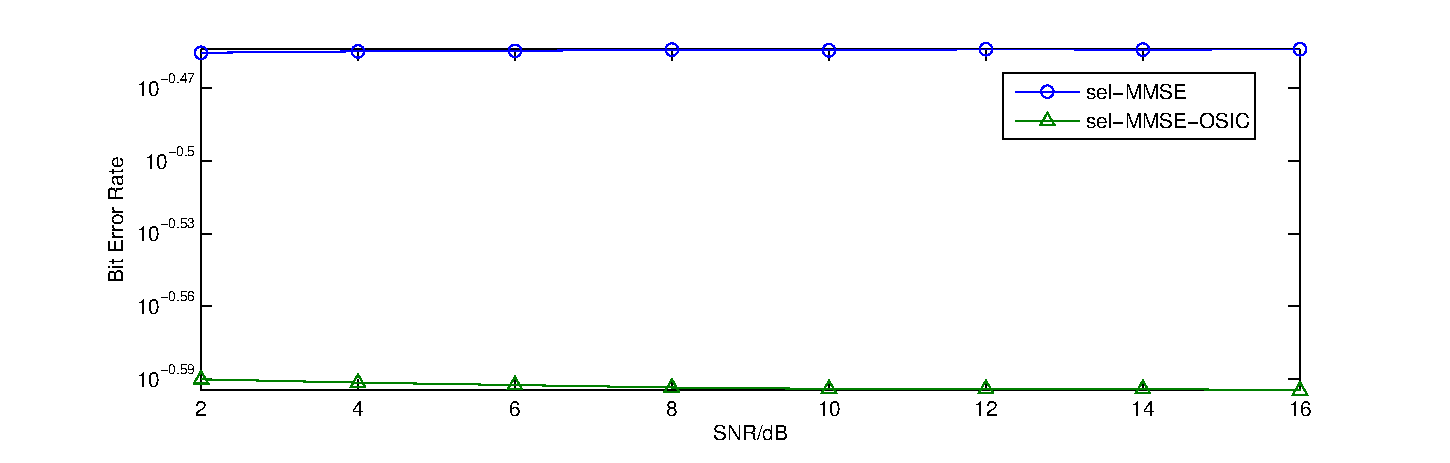
\includegraphics[scale=0.8]{hardening.eps}
\caption{BER performance of sel-MMSE and sel-MMSE-OSIC with channel hardening phenomenon}
\label{figure1}
\end{figure} \\
Consider MMSE algorithm:
 \begin{equation}
 \hat{s}=\mathbf{G}y=\mathbf{G}\mathbf{H}s+\mathbf{G}n    \label{future1}
 \end{equation}
the definitions of $\mathbf{H}$ $y$ $s$ $n$ $\hat{s}$ are similar to the definitions in section \ref{system}. $G=(\mathbf{H}^{H}\mathbf{H}+SNR^{-1})^{-1}\mathbf{H}^{H}$ is the weight matrix, define $\mathbf{C}=(\mathbf{H}^{H}\mathbf{H}+SNR^{-1})^{-1}$. From (\ref{future1}) we have:
 \begin{equation}
\hat{s}_{k}=c_{kk}\mathbf{H}^{H}\mathbf{H}s+c_{kk}\mathbf{H}^{H}n+\sum_{j\neq k}c_{kj}\mathbf{H}^{H}\mathbf{H}s+\sum_{j\neq k}c_{kj}\mathbf{H}^{H}n \label{future2}
\end{equation}
$k\in [1,N_{t}]$, $\hat{s}_{k}$ is the $k$th element of $\hat{s}$, $c_{kj}$ is the element of $\mathbf{C}$ at $k$th row and $j$th column.
with channel hardening phenomenon (\ref{future2}) is changed to:
\begin{equation}
\hat{s}_{k}^{hardening}=\frac{1}{N_{r}+SNR^{-1}}\mathbf{H}^{H}\mathbf{H}s+\frac{1}{N_{r}+SNR^{-1}}\mathbf{H}^{H}n\label{future3}
\end{equation}
$\hat{s}_{k}^{hardening}$ is the MMSE estimation with channel hardening phenomenon applied.
comparing (\ref{future2}) and (\ref{future3}), the off diagonal elements of $\mathbf{C}$ is ignored in (\ref{future3}), with the fixed $N_{r}$ if $N_{t}$ increases, the number of off diagonal elements of $\mathbf{C}$ increases and performance get worse, so it is not reasonable to ignore them. This explain the result in Figure.\ref{figure1}, this kind of inter user interference(IUI) causes performance lost. Therefore, the next step is to find a strategy to eliminate this IUI without increasing too much complexity.
% conference papers do not normally have an appendix


% use section* for acknowledgement
%\section*{Acknowledgment}








% trigger a \newpage just before the given reference
% number - used to balance the columns on the last page
% adjust value as needed - may need to be readjusted if
% the document is modified later
%\IEEEtriggeratref{8}
% The "triggered" command can be changed if desired:
%\IEEEtriggercmd{\enlargethispage{-5in}}

% references section

% can use a bibliography generated by BibTeX as a .bbl file
% BibTeX documentation can be easily obtained at:
% http://www.ctan.org/tex-archive/biblio/bibtex/contrib/doc/
% The IEEEtran BibTeX style support page is at:
% http://www.michaelshell.org/tex/ieeetran/bibtex/
%\bibliographystyle{IEEEtran}
% argument is your BibTeX string definitions and bibliography database(s)
%\bibliography{IEEEabrv,../bib/paper}
%
% <OR> manually copy in the resultant .bbl file
% set second argument of \begin to the number of references
% (used to reserve space for the reference number labels box)






% that's all folks
\end{spacing}
\bibliographystyle{IEEEtran}
\bibliography{citation}
\end{document}


